% L13c figure: one tool call, from the user's question to the answer.
%
% Four lifelines: the language model, the host, the MCP server, and the web
% API. The host gives the model the question and the tool list (1); the model
% picks a tool and its arguments (2); the host sends a tools/call request (3);
% the server calls the web API (4, 5); the server returns the result (6); the
% host gives the result to the model (7); the model writes the answer (8).
% Blue arrows are MCP messages, dark arrows are HTTPS, gray arrows stay
% inside the host application.
%
% Drawn on November 12, 2026 with the palette and build of the L13a figures.
% The notebook SVG carries a dark palette added by theme_svg.py; keep new
% colors in that script's mapping when changing the palette here.
\documentclass[tikz,border=4pt]{standalone}
\usepackage[no-math]{fontspec}
\IfFontExistsTF{Arial}{\setsansfont{Arial}}{\setsansfont{TeX Gyre Heros}}
\renewcommand{\familydefault}{\sfdefault}
\usepackage{amsmath,amssymb}
\usetikzlibrary{arrows.meta, calc}

% Ink, blue, gray, and band match the L13a figures. Blue marks the MCP messages.
\definecolor{vnink}{HTML}{202124}
\definecolor{gdblue}{HTML}{0091FF}
\definecolor{gdgray}{HTML}{6D7278}
\definecolor{waband}{HTML}{EEF0F2}
\definecolor{nodefill}{HTML}{FFFFFF}

\begin{document}
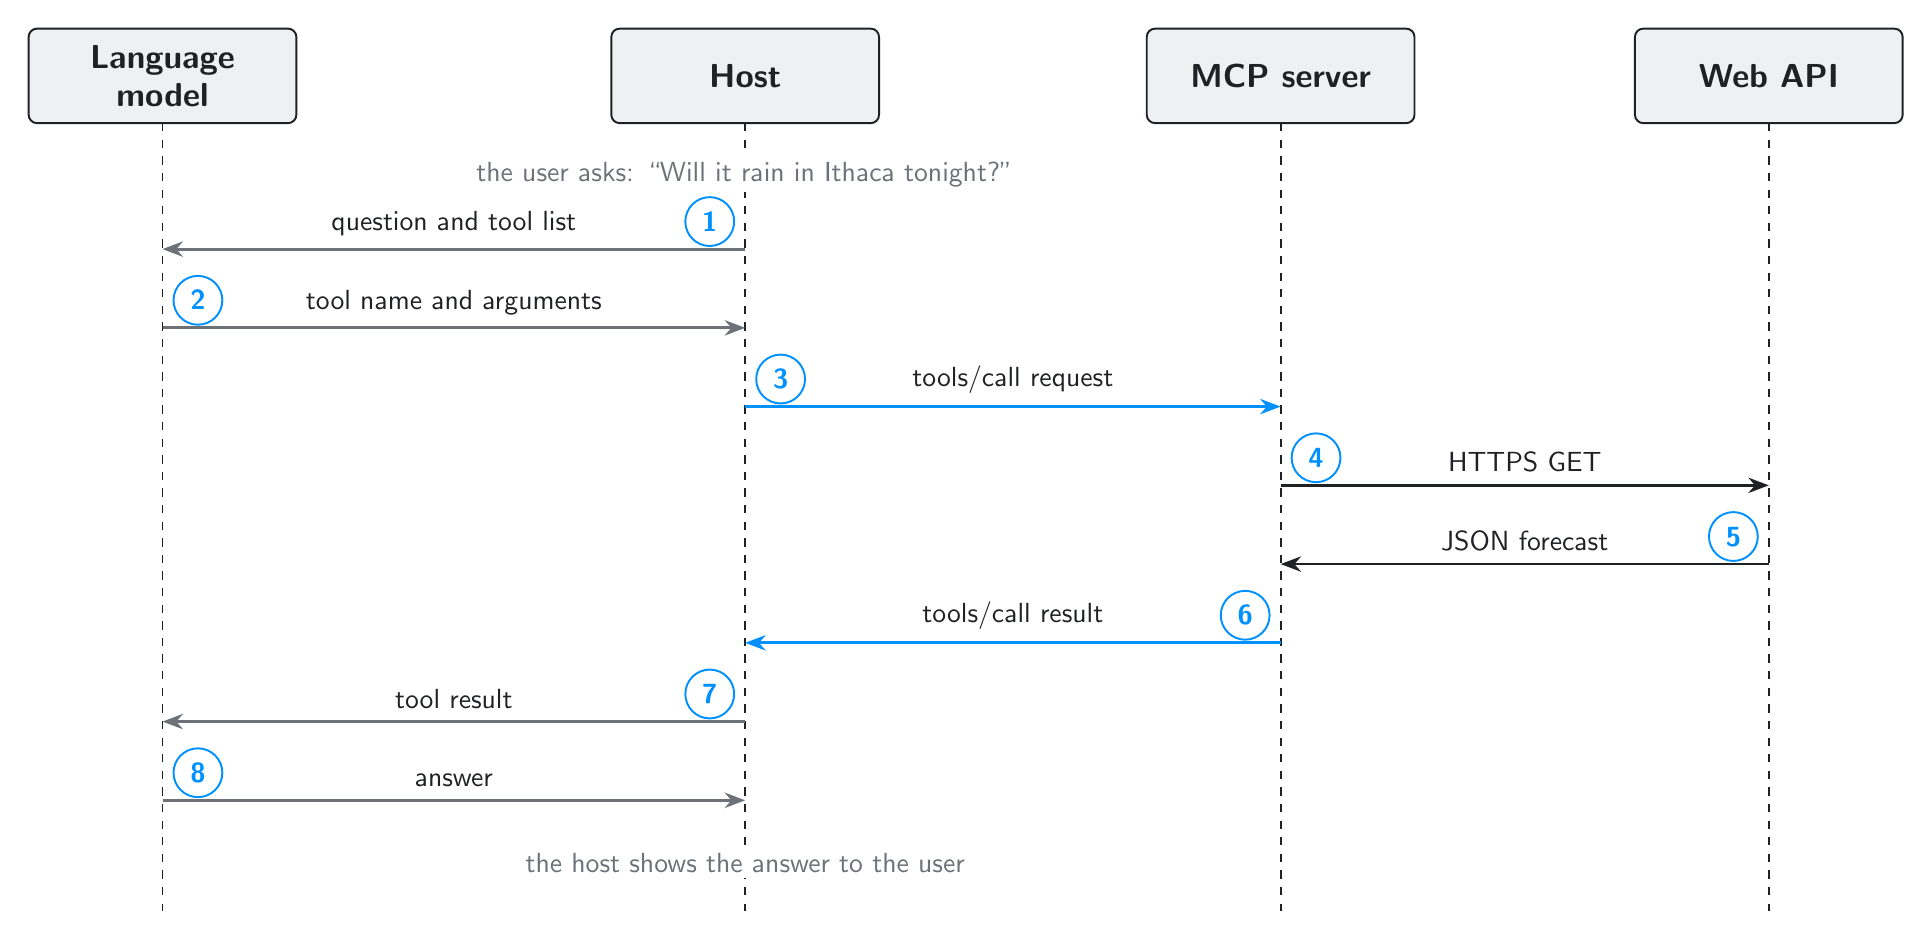
\begin{tikzpicture}[
  font=\sffamily\large,
  >={Stealth[length=2.6mm]},
  head/.style={draw=vnink, rounded corners=3pt, minimum width=3.4cm, minimum height=1.2cm,
    fill=waband, line width=0.7pt, text=vnink, align=center, font=\sffamily\large\bfseries},
  life/.style={line width=0.7pt, draw=vnink, dashed},
  msg/.style={font=\sffamily\normalsize, text=vnink, align=center},
  note/.style={font=\sffamily\normalsize, text=gdgray, align=center},
  stepnum/.style={circle, draw=gdblue, fill=nodefill, line width=0.7pt, inner sep=0pt,
    minimum size=6.2mm, font=\sffamily\normalsize\bfseries, text=gdblue},
  mcp/.style={->, line width=1.0pt, draw=gdblue},
  https/.style={->, line width=1.0pt, draw=vnink},
  local/.style={->, line width=1.0pt, draw=gdgray}
]

% x positions of the four lifelines, and the y position of each step -
\def\xM{0.0}
\def\xH{7.4}
\def\xS{14.2}
\def\xA{20.4}

% ------------------------------------------------------------ headers and lifelines
\node[head] (m) at (\xM, 0) {Language\\model};
\node[head] (h) at (\xH, 0) {Host};
\node[head] (s) at (\xS, 0) {MCP server};
\node[head] (a) at (\xA, 0) {Web API};
\foreach \x in {\xM, \xH, \xS, \xA} {
  \draw[life] (\x, -0.6) -- (\x, -10.6);
}

% the question arrives at the host -
\node[note, fill=nodefill, inner sep=2pt] at (\xH, -1.25) {the user asks: ``Will it rain in Ithaca tonight?''};

% ------------------------------------------------------------ the eight steps
% 1: the host gives the model the question and the tool list
\draw[local] (\xH, -2.2) -- (\xM, -2.2) node[msg, midway, above=1pt] {question and tool list};
\node[stepnum] at (\xH - 0.45, -1.85) {1};

% 2: the model picks a tool and its arguments
\draw[local] (\xM, -3.2) -- (\xH, -3.2) node[msg, midway, above=1pt] {tool name and arguments};
\node[stepnum] at (\xM + 0.45, -2.85) {2};

% 3: the host sends a tools/call request to the server
\draw[mcp] (\xH, -4.2) -- (\xS, -4.2) node[msg, midway, above=1pt] {tools/call request};
\node[stepnum] at (\xH + 0.45, -3.85) {3};

% 4: the server calls the web API
\draw[https] (\xS, -5.2) -- (\xA, -5.2) node[msg, midway, above=1pt] {HTTPS GET};
\node[stepnum] at (\xS + 0.45, -4.85) {4};

% 5: the web API answers
\draw[https] (\xA, -6.2) -- (\xS, -6.2) node[msg, midway, above=1pt] {JSON forecast};
\node[stepnum] at (\xA - 0.45, -5.85) {5};

% 6: the server returns the result of the tool
\draw[mcp] (\xS, -7.2) -- (\xH, -7.2) node[msg, midway, above=1pt] {tools/call result};
\node[stepnum] at (\xS - 0.45, -6.85) {6};

% 7: the host gives the result to the model
\draw[local] (\xH, -8.2) -- (\xM, -8.2) node[msg, midway, above=1pt] {tool result};
\node[stepnum] at (\xH - 0.45, -7.85) {7};

% 8: the model writes the answer
\draw[local] (\xM, -9.2) -- (\xH, -9.2) node[msg, midway, above=1pt] {answer};
\node[stepnum] at (\xM + 0.45, -8.85) {8};

% the host shows the answer -
\node[note, fill=nodefill, inner sep=2pt] at (\xH, -10.0) {the host shows the answer to the user};

\end{tikzpicture}
\end{document}
